%%%%
\documentclass[10pt]{report}
\usepackage{graphicx,color,epsfig,psfig,subfigure}
\usepackage{amsmath,amsfonts,amssymb}
\usepackage{bm}
\pagestyle{empty}
\begin{document}
\begin{picture}(0,0)%
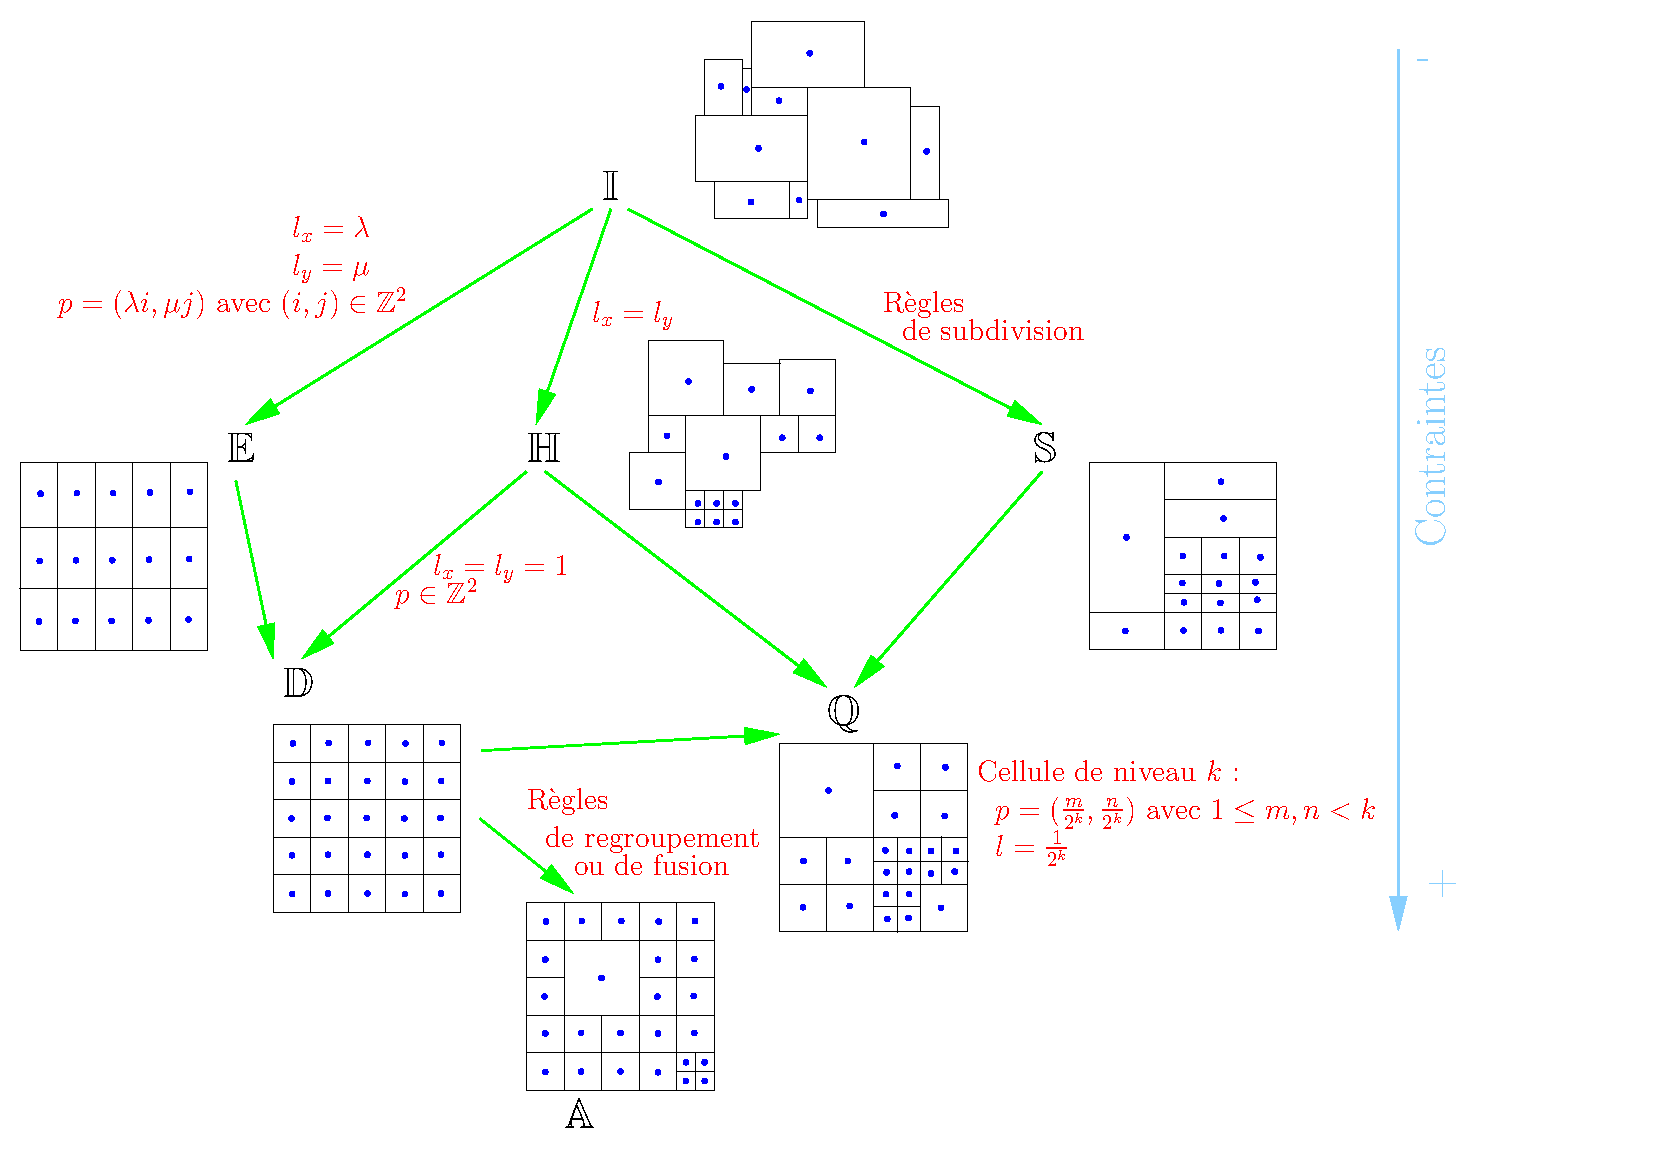
\includegraphics{schemabis.pstex}%
\end{picture}%
\setlength{\unitlength}{3947sp}%
%
\begingroup\makeatletter\ifx\SetFigFontNFSS\undefined%
\gdef\SetFigFontNFSS#1#2#3#4#5{%
  \reset@font\fontsize{#1}{#2pt}%
  \fontfamily{#3}\fontseries{#4}\fontshape{#5}%
  \selectfont}%
\fi\endgroup%
\begin{picture}(11469,8967)(-169,-7966)
\put(7501,-5086){\makebox(0,0)[lb]{\smash{{\SetFigFontNFSS{14}{16.8}{\familydefault}{\mddefault}{\updefault}{\color[rgb]{1,0,0}Cellule de niveau $k$ :}%
}}}}
\put(7651,-5686){\makebox(0,0)[lb]{\smash{{\SetFigFontNFSS{14}{16.8}{\familydefault}{\mddefault}{\updefault}{\color[rgb]{1,0,0}$l=\frac{1}{2^ k}$}%
}}}}
\put(7651,-5386){\makebox(0,0)[lb]{\smash{{\SetFigFontNFSS{14}{16.8}{\familydefault}{\mddefault}{\updefault}{\color[rgb]{1,0,0}$p=(\frac{m}{2^k},\frac{n}{2^k})$ avec $1\leq m,n< k$}%
}}}}
\put(7951,-2536){\makebox(0,0)[lb]{\smash{{\SetFigFontNFSS{20}{24.0}{\familydefault}{\mddefault}{\updefault}{\color[rgb]{0,0,0}$\mathbb{S}$}%
}}}}
\put(6901,-1561){\makebox(0,0)[lb]{\smash{{\SetFigFontNFSS{14}{16.8}{\familydefault}{\mddefault}{\updefault}{\color[rgb]{1,0,0}de subdivisions}%
}}}}
\put(4426,-1411){\makebox(0,0)[lb]{\smash{{\SetFigFontNFSS{14}{16.8}{\familydefault}{\mddefault}{\updefault}{\color[rgb]{1,0,0}$l_x=l_y$}%
}}}}
\put(4501,-436){\makebox(0,0)[lb]{\smash{{\SetFigFontNFSS{20}{24.0}{\familydefault}{\mddefault}{\updefault}{\color[rgb]{0,0,0}$\mathbb{I}$}%
}}}}
\put(2851,-3661){\makebox(0,0)[lb]{\smash{{\SetFigFontNFSS{14}{16.8}{\familydefault}{\mddefault}{\updefault}{\color[rgb]{1,0,0}$p \in \mathbb{Z}^2$}%
}}}}
\put(1951,-4411){\makebox(0,0)[lb]{\smash{{\SetFigFontNFSS{20}{24.0}{\familydefault}{\mddefault}{\updefault}{\color[rgb]{0,0,0}$\mathbb{D}$}%
}}}}
\put(1501,-2536){\makebox(0,0)[lb]{\smash{{\SetFigFontNFSS{20}{24.0}{\familydefault}{\mddefault}{\updefault}{\color[rgb]{0,0,0}$\mathbb{E}$}%
}}}}
\put(6751,-1336){\makebox(0,0)[lb]{\smash{{\SetFigFontNFSS{14}{16.8}{\familydefault}{\mddefault}{\updefault}{\color[rgb]{1,0,0}R\`egles}%
}}}}
\put(3151,-3436){\makebox(0,0)[lb]{\smash{{\SetFigFontNFSS{14}{16.8}{\familydefault}{\mddefault}{\updefault}{\color[rgb]{1,0,0}$l_x=l_y=1$}%
}}}}
\put(6301,-4636){\makebox(0,0)[lb]{\smash{{\SetFigFontNFSS{20}{24.0}{\familydefault}{\mddefault}{\updefault}{\color[rgb]{0,0,0}$\mathbb{Q}$}%
}}}}
\put(2026,-1036){\makebox(0,0)[lb]{\smash{{\SetFigFontNFSS{14}{16.8}{\familydefault}{\mddefault}{\updefault}{\color[rgb]{1,0,0}$l_y=\mu$}%
}}}}
\put(2026,-736){\makebox(0,0)[lb]{\smash{{\SetFigFontNFSS{14}{16.8}{\familydefault}{\mddefault}{\updefault}{\color[rgb]{1,0,0}$l_x=\lambda$}%
}}}}
\put(151,-1336){\makebox(0,0)[lb]{\smash{{\SetFigFontNFSS{14}{16.8}{\familydefault}{\mddefault}{\updefault}{\color[rgb]{1,0,0}$p=(\lambda i,\mu j)$ avec $(i,j)\in\mathbb{Z}^2$}%
}}}}
\put(11251,-3211){\rotatebox{90.0}{\makebox(0,0)[lb]{\smash{{\SetFigFontNFSS{20}{24.0}{\familydefault}{\mddefault}{\updefault}{\color[rgb]{.53,.81,1}Contraintes}%
}}}}}
\put(11026,614){\makebox(0,0)[lb]{\smash{{\SetFigFontNFSS{20}{24.0}{\familydefault}{\mddefault}{\updefault}{\color[rgb]{.53,.81,1}-}%
}}}}
\put(11101,-5986){\makebox(0,0)[lb]{\smash{{\SetFigFontNFSS{20}{24.0}{\familydefault}{\mddefault}{\updefault}{\color[rgb]{.53,.81,1}+}%
}}}}
\put(4201,-7861){\makebox(0,0)[lb]{\smash{{\SetFigFontNFSS{20}{24.0}{\familydefault}{\mddefault}{\updefault}{\color[rgb]{0,0,0}$\mathbb{A}$}%
}}}}
\put(3901,-5311){\makebox(0,0)[lb]{\smash{{\SetFigFontNFSS{14}{16.8}{\familydefault}{\mddefault}{\updefault}{\color[rgb]{1,0,0}R\`egles}%
}}}}
\put(4051,-5611){\makebox(0,0)[lb]{\smash{{\SetFigFontNFSS{14}{16.8}{\familydefault}{\mddefault}{\updefault}{\color[rgb]{1,0,0}de regroupement}%
}}}}
\put(4276,-5836){\makebox(0,0)[lb]{\smash{{\SetFigFontNFSS{14}{16.8}{\familydefault}{\mddefault}{\updefault}{\color[rgb]{1,0,0}ou de fusion}%
}}}}
\put(3901,-2536){\makebox(0,0)[lb]{\smash{{\SetFigFontNFSS{20}{24.0}{\familydefault}{\mddefault}{\updefault}{\color[rgb]{0,0,0}$\mathbb{H}$}%
}}}}
\end{picture}%
\end{document}
